\chapter{The Power of (Percieved) Media Bias}





Why is media bias IMPORTANT? Why is the problem IMPORTANT?

 
- Fox News Effect
- Does the media matter


\section{The Role of the Reader in Perceptions of Bias}

It comes as no surprise that our own political stances have a significant effect in our perceptions of bias in the media. 

In even seemingly neutral stories, partisans tend to view reporting as biased against their own views. This phenomenon-- deemed the ``hostile media effect''-- was first studied at Stanford University by Robert P. Vallone, Lee Ross, and Mark R. Lepper in 1985 \cite{vallone1985hostile}. Although ``true'' neutrality of a story is nearly impossible to quantify due to the subjective nature of the concept, Vallone et. al were able to successfully demonstrate that partisans of \emph{both} sides (pro-Israeli and pro-Arab) viewed the same news segments as hostile towards their beliefs and favorable to the other side.

? Perceptions of media bias, then, have as much to do as self-serving motivations to secure preferential treatment as they do with the media itself.
  
? The political leanings of the reader are essential considerations when attempting to measure other factors that contribute to bias. In 

\section{The Role of Media Brands in Perceptions of Bias}
The media, of course, is not just one unified mass, and in an increasingly fragmented ecosystem, the role of media brands is a crucial factor in the perception of bias. Although most research
\cite{baum2008eye}








For instance, most research on the hostile media phenomenon conceptualizes the news media as an undifferentiated mass of information sources that individuals can (and do) reasonably characterize as having a uniform political orientation (Giner-Sorolla and Chaiken 1994, Peffley et al. 2001, Eveland and Shah 2003). Yet, the past two decades have seen a dramatic increase in the number and variety of news sources. One consequence is that Democrats and Republicans are increasingly likely to differ systematically in their assessments of specific media outlets.






With the decline of print newspapers, a diverse number of new platforms and web-centric publications have risen.


How do you control for the above things in your study?

\section{The Role of Language [Policial Persuasion]}




\subsection{Language and Politics}
Presidential speeches degrading over time-- ie simple language appeals to the masses in politics
\subsection{The Seductive Allure [... of Simple] Language}
But we trust complex language for explaining technical facts

Test image

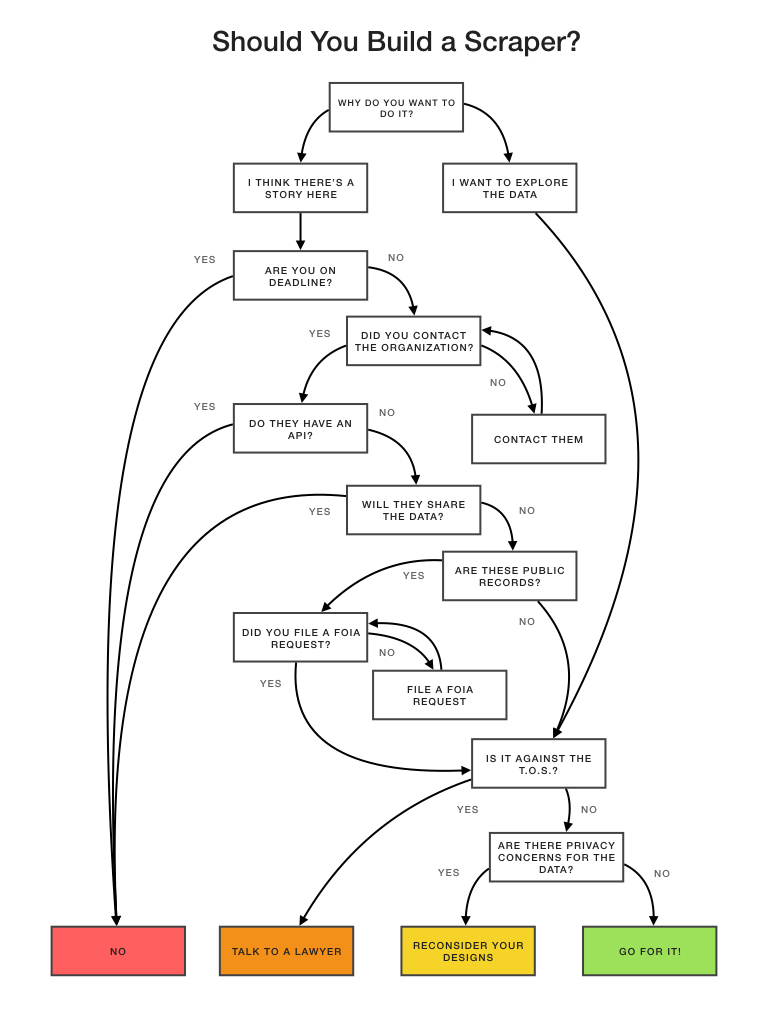
\includegraphics[width=\textwidth]{flowchart_final}


\section{Importance in Political Outcomes}
Fox news effect 

\section{The 2016 Elections} 
\subsection{Criticism of Media Bias} 
(Obama Speech)

So.... are you what you cover?








